\documentclass[twoside]{book}

% Packages required by doxygen
\usepackage{fixltx2e}
\usepackage{calc}
\usepackage{doxygen}
\usepackage[export]{adjustbox} % also loads graphicx
\usepackage{graphicx}
\usepackage[utf8]{inputenc}
\usepackage{makeidx}
\usepackage{multicol}
\usepackage{multirow}
\PassOptionsToPackage{warn}{textcomp}
\usepackage{textcomp}
\usepackage[nointegrals]{wasysym}
\usepackage[table]{xcolor}

% Font selection
\usepackage[T1]{fontenc}
\usepackage[scaled=.90]{helvet}
\usepackage{courier}
\usepackage{amssymb}
\usepackage{sectsty}
\renewcommand{\familydefault}{\sfdefault}
\allsectionsfont{%
  \fontseries{bc}\selectfont%
  \color{darkgray}%
}
\renewcommand{\DoxyLabelFont}{%
  \fontseries{bc}\selectfont%
  \color{darkgray}%
}
\newcommand{\+}{\discretionary{\mbox{\scriptsize$\hookleftarrow$}}{}{}}

% Page & text layout
\usepackage{geometry}
\geometry{%
  a4paper,%
  top=2.5cm,%
  bottom=2.5cm,%
  left=2.5cm,%
  right=2.5cm%
}
\tolerance=750
\hfuzz=15pt
\hbadness=750
\setlength{\emergencystretch}{15pt}
\setlength{\parindent}{0cm}
\setlength{\parskip}{3ex plus 2ex minus 2ex}
\makeatletter
\renewcommand{\paragraph}{%
  \@startsection{paragraph}{4}{0ex}{-1.0ex}{1.0ex}{%
    \normalfont\normalsize\bfseries\SS@parafont%
  }%
}
\renewcommand{\subparagraph}{%
  \@startsection{subparagraph}{5}{0ex}{-1.0ex}{1.0ex}{%
    \normalfont\normalsize\bfseries\SS@subparafont%
  }%
}
\makeatother

% Headers & footers
\usepackage{fancyhdr}
\pagestyle{fancyplain}
\fancyhead[LE]{\fancyplain{}{\bfseries\thepage}}
\fancyhead[CE]{\fancyplain{}{}}
\fancyhead[RE]{\fancyplain{}{\bfseries\leftmark}}
\fancyhead[LO]{\fancyplain{}{\bfseries\rightmark}}
\fancyhead[CO]{\fancyplain{}{}}
\fancyhead[RO]{\fancyplain{}{\bfseries\thepage}}
\fancyfoot[LE]{\fancyplain{}{}}
\fancyfoot[CE]{\fancyplain{}{}}
\fancyfoot[RE]{\fancyplain{}{\bfseries\scriptsize Generated by Doxygen }}
\fancyfoot[LO]{\fancyplain{}{\bfseries\scriptsize Generated by Doxygen }}
\fancyfoot[CO]{\fancyplain{}{}}
\fancyfoot[RO]{\fancyplain{}{}}
\renewcommand{\footrulewidth}{0.4pt}
\renewcommand{\chaptermark}[1]{%
  \markboth{#1}{}%
}
\renewcommand{\sectionmark}[1]{%
  \markright{\thesection\ #1}%
}

% Indices & bibliography
\usepackage{natbib}
\usepackage[titles]{tocloft}
\setcounter{tocdepth}{3}
\setcounter{secnumdepth}{5}
\makeindex

% Hyperlinks (required, but should be loaded last)
\usepackage{ifpdf}
\ifpdf
  \usepackage[pdftex,pagebackref=true]{hyperref}
\else
  \usepackage[ps2pdf,pagebackref=true]{hyperref}
\fi
\hypersetup{%
  colorlinks=true,%
  linkcolor=blue,%
  citecolor=blue,%
  unicode%
}

% Custom commands
\newcommand{\clearemptydoublepage}{%
  \newpage{\pagestyle{empty}\cleardoublepage}%
}

\usepackage{caption}
\captionsetup{labelsep=space,justification=centering,font={bf},singlelinecheck=off,skip=4pt,position=top}

%===== C O N T E N T S =====

\begin{document}

% Titlepage & ToC
\hypersetup{pageanchor=false,
             bookmarksnumbered=true,
             pdfencoding=unicode
            }
\pagenumbering{alph}
\begin{titlepage}
\vspace*{7cm}
\begin{center}%
{\Large My Project }\\
\vspace*{1cm}
{\large Generated by Doxygen 1.8.14}\\
\end{center}
\end{titlepage}
\clearemptydoublepage
\pagenumbering{roman}
\tableofcontents
\clearemptydoublepage
\pagenumbering{arabic}
\hypersetup{pageanchor=true}

%--- Begin generated contents ---
\chapter{Hierarchical Index}
\section{Class Hierarchy}
This inheritance list is sorted roughly, but not completely, alphabetically\+:\begin{DoxyCompactList}
\item \contentsline{section}{trivia.\+App}{\pageref{classtrivia_1_1App}}{}
\item Model\begin{DoxyCompactList}
\item \contentsline{section}{trivia.\+Game}{\pageref{classtrivia_1_1Game}}{}
\item \contentsline{section}{trivia.\+Question}{\pageref{classtrivia_1_1Question}}{}
\item \contentsline{section}{trivia.\+Respondida}{\pageref{classtrivia_1_1Respondida}}{}
\item \contentsline{section}{trivia.\+User}{\pageref{classtrivia_1_1User}}{}
\begin{DoxyCompactList}
\item \contentsline{section}{trivia.\+Admin}{\pageref{classtrivia_1_1Admin}}{}
\end{DoxyCompactList}
\end{DoxyCompactList}
\end{DoxyCompactList}

\chapter{Class Index}
\section{Class List}
Here are the classes, structs, unions and interfaces with brief descriptions\+:\begin{DoxyCompactList}
\item\contentsline{section}{\mbox{\hyperlink{classtrivia_1_1Admin}{trivia.\+Admin}} }{\pageref{classtrivia_1_1Admin}}{}
\item\contentsline{section}{\mbox{\hyperlink{classtrivia_1_1App}{trivia.\+App}} }{\pageref{classtrivia_1_1App}}{}
\item\contentsline{section}{\mbox{\hyperlink{classtrivia_1_1Game}{trivia.\+Game}} }{\pageref{classtrivia_1_1Game}}{}
\item\contentsline{section}{\mbox{\hyperlink{classtrivia_1_1Question}{trivia.\+Question}} }{\pageref{classtrivia_1_1Question}}{}
\item\contentsline{section}{\mbox{\hyperlink{classtrivia_1_1Respondida}{trivia.\+Respondida}} }{\pageref{classtrivia_1_1Respondida}}{}
\item\contentsline{section}{\mbox{\hyperlink{classtrivia_1_1User}{trivia.\+User}} }{\pageref{classtrivia_1_1User}}{}
\end{DoxyCompactList}

\chapter{Class Documentation}
\hypertarget{classtrivia_1_1Admin}{}\section{trivia.\+Admin Class Reference}
\label{classtrivia_1_1Admin}\index{trivia.\+Admin@{trivia.\+Admin}}
Inheritance diagram for trivia.\+Admin\+:\begin{figure}[H]
\begin{center}
\leavevmode
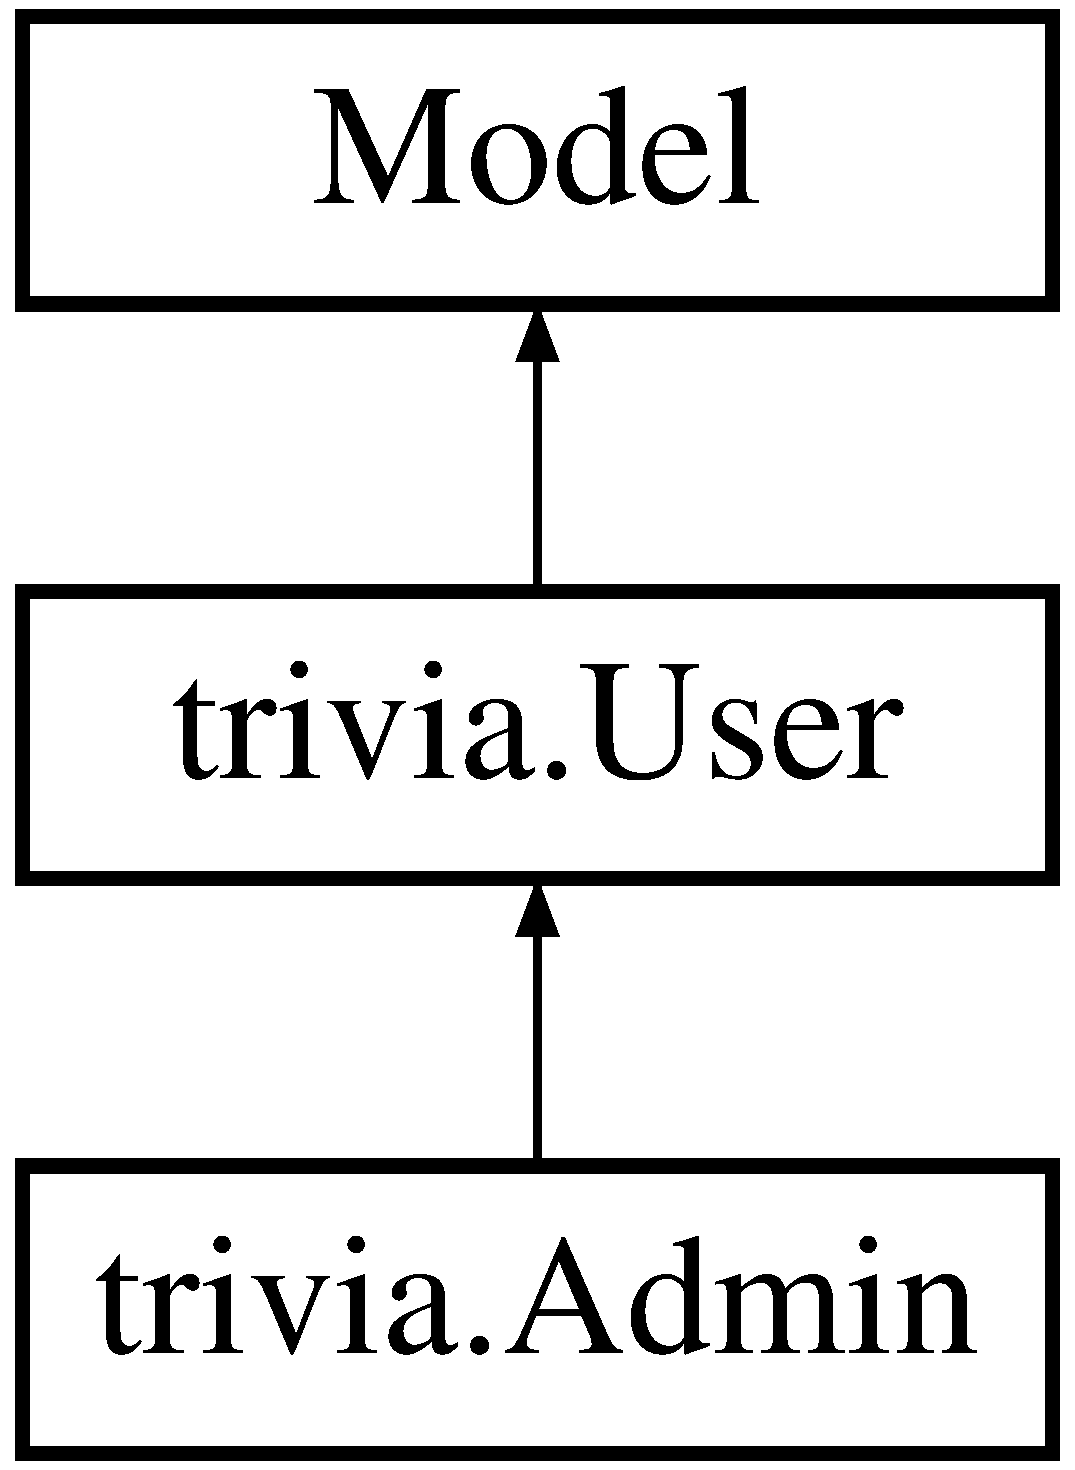
\includegraphics[height=3.000000cm]{classtrivia_1_1Admin}
\end{center}
\end{figure}
\subsection*{Additional Inherited Members}


\subsection{Detailed Description}
Clase \mbox{\hyperlink{classtrivia_1_1Admin}{Admin}}, extiende de \mbox{\hyperlink{classtrivia_1_1User}{User}} para poder logearse y por tanto tambien de Model. 

The documentation for this class was generated from the following file\+:\begin{DoxyCompactItemize}
\item 
Admin.\+java\end{DoxyCompactItemize}

\hypertarget{classtrivia_1_1App}{}\section{trivia.\+App Class Reference}
\label{classtrivia_1_1App}\index{trivia.\+App@{trivia.\+App}}
\subsection*{Static Public Member Functions}
\begin{DoxyCompactItemize}
\item 
\mbox{\Hypertarget{classtrivia_1_1App_ad2da3a023757541d9eecc0a10a213168}\label{classtrivia_1_1App_ad2da3a023757541d9eecc0a10a213168}} 
static void {\bfseries main} (String\mbox{[}$\,$\mbox{]} args)
\item 
static int \mbox{\hyperlink{classtrivia_1_1App_adcedb003b5a5fa73689c3d7a276f9530}{rand\+Int}} (int min, int max)
\item 
static void \mbox{\hyperlink{classtrivia_1_1App_a626312af5afd16555429d2241273d85d}{open\+DB}} ()
\item 
static void \mbox{\hyperlink{classtrivia_1_1App_a32815da15f55607f228ee3a431c98e46}{close\+DB}} ()
\item 
static boolean \mbox{\hyperlink{classtrivia_1_1App_a0ba549b8577987ac6565b91ad65d6cce}{existe\+Host}} (String host\+Name)
\item 
static void \mbox{\hyperlink{classtrivia_1_1App_a4753bc6610d49e0d101c01d00b4b99d6}{close\+Host}} (String usuario\+Creador)
\end{DoxyCompactItemize}


\subsection{Detailed Description}
Clase Principal que administra el juego y sus subprocesos. \begin{DoxyAuthor}{Author}
Maria, Santiago; Rivero, Matias. 
\end{DoxyAuthor}
\begin{DoxyVersion}{Version}
0.\+5 
\end{DoxyVersion}


\subsection{Member Function Documentation}
\mbox{\Hypertarget{classtrivia_1_1App_a32815da15f55607f228ee3a431c98e46}\label{classtrivia_1_1App_a32815da15f55607f228ee3a431c98e46}} 
\index{trivia\+::\+App@{trivia\+::\+App}!close\+DB@{close\+DB}}
\index{close\+DB@{close\+DB}!trivia\+::\+App@{trivia\+::\+App}}
\subsubsection{\texorpdfstring{close\+D\+B()}{closeDB()}}
{\footnotesize\ttfamily static void trivia.\+App.\+close\+DB (\begin{DoxyParamCaption}{ }\end{DoxyParamCaption})\hspace{0.3cm}{\ttfamily [inline]}, {\ttfamily [static]}}

Metodo que intenta cerrar la conexion a la base de datos. \begin{DoxyAuthor}{Author}
Maria, Santiago; Rivero, Matias. 
\end{DoxyAuthor}
\mbox{\Hypertarget{classtrivia_1_1App_a4753bc6610d49e0d101c01d00b4b99d6}\label{classtrivia_1_1App_a4753bc6610d49e0d101c01d00b4b99d6}} 
\index{trivia\+::\+App@{trivia\+::\+App}!close\+Host@{close\+Host}}
\index{close\+Host@{close\+Host}!trivia\+::\+App@{trivia\+::\+App}}
\subsubsection{\texorpdfstring{close\+Host()}{closeHost()}}
{\footnotesize\ttfamily static void trivia.\+App.\+close\+Host (\begin{DoxyParamCaption}\item[{String}]{usuario\+Creador }\end{DoxyParamCaption})\hspace{0.3cm}{\ttfamily [inline]}, {\ttfamily [static]}}

Metodo estatico que cierra la partida que tiene por creador al usuario cuyo nombre es pasado como parametro. \begin{DoxyAuthor}{Author}
Maria, Santiago; Rivero, Matias. 
\end{DoxyAuthor}

\begin{DoxyParams}{Parameters}
{\em usuario\+Creador} & nombre de usuario del creador de la partida que se desea cerrar. \\
\hline
\end{DoxyParams}
\mbox{\Hypertarget{classtrivia_1_1App_a0ba549b8577987ac6565b91ad65d6cce}\label{classtrivia_1_1App_a0ba549b8577987ac6565b91ad65d6cce}} 
\index{trivia\+::\+App@{trivia\+::\+App}!existe\+Host@{existe\+Host}}
\index{existe\+Host@{existe\+Host}!trivia\+::\+App@{trivia\+::\+App}}
\subsubsection{\texorpdfstring{existe\+Host()}{existeHost()}}
{\footnotesize\ttfamily static boolean trivia.\+App.\+existe\+Host (\begin{DoxyParamCaption}\item[{String}]{host\+Name }\end{DoxyParamCaption})\hspace{0.3cm}{\ttfamily [inline]}, {\ttfamily [static]}}

Metodo estatico booleano que retorna true si el hostname pasado como parametro ya esta siendo usado por otro usuario. \begin{DoxyAuthor}{Author}
Maria, Santiago; Rivero, Matias. 
\end{DoxyAuthor}

\begin{DoxyParams}{Parameters}
{\em host\+Name} & nombre de la partida que se desea crear, la cual es controlada para que no existan dos partidas con el mismo nombre. \\
\hline
\end{DoxyParams}
\mbox{\Hypertarget{classtrivia_1_1App_a626312af5afd16555429d2241273d85d}\label{classtrivia_1_1App_a626312af5afd16555429d2241273d85d}} 
\index{trivia\+::\+App@{trivia\+::\+App}!open\+DB@{open\+DB}}
\index{open\+DB@{open\+DB}!trivia\+::\+App@{trivia\+::\+App}}
\subsubsection{\texorpdfstring{open\+D\+B()}{openDB()}}
{\footnotesize\ttfamily static void trivia.\+App.\+open\+DB (\begin{DoxyParamCaption}{ }\end{DoxyParamCaption})\hspace{0.3cm}{\ttfamily [inline]}, {\ttfamily [static]}}

Metodo que intenta abrir una conexion a la base de datos. \begin{DoxyAuthor}{Author}
Maria, Santiago; Rivero, Matias. 
\end{DoxyAuthor}
\mbox{\Hypertarget{classtrivia_1_1App_adcedb003b5a5fa73689c3d7a276f9530}\label{classtrivia_1_1App_adcedb003b5a5fa73689c3d7a276f9530}} 
\index{trivia\+::\+App@{trivia\+::\+App}!rand\+Int@{rand\+Int}}
\index{rand\+Int@{rand\+Int}!trivia\+::\+App@{trivia\+::\+App}}
\subsubsection{\texorpdfstring{rand\+Int()}{randInt()}}
{\footnotesize\ttfamily static int trivia.\+App.\+rand\+Int (\begin{DoxyParamCaption}\item[{int}]{min,  }\item[{int}]{max }\end{DoxyParamCaption})\hspace{0.3cm}{\ttfamily [inline]}, {\ttfamily [static]}}

Returns a pseudo-\/random number between min and max, inclusive. The difference between min and max can be at most {\ttfamily Integer.\+M\+A\+X\+\_\+\+V\+A\+L\+UE -\/ 1}.


\begin{DoxyParams}{Parameters}
{\em min} & Minimum value \\
\hline
{\em max} & Maximum value. Must be greater than min. \\
\hline
\end{DoxyParams}
\begin{DoxyReturn}{Returns}
Integer between min and max, inclusive. 
\end{DoxyReturn}
\begin{DoxySeeAlso}{See also}
java.\+util.\+Random\+::next\+Int(int) 
\end{DoxySeeAlso}


The documentation for this class was generated from the following file\+:\begin{DoxyCompactItemize}
\item 
App.\+java\end{DoxyCompactItemize}

\hypertarget{classtrivia_1_1Game}{}\section{trivia.\+Game Class Reference}
\label{classtrivia_1_1Game}\index{trivia.\+Game@{trivia.\+Game}}
Inheritance diagram for trivia.\+Game\+:\begin{figure}[H]
\begin{center}
\leavevmode
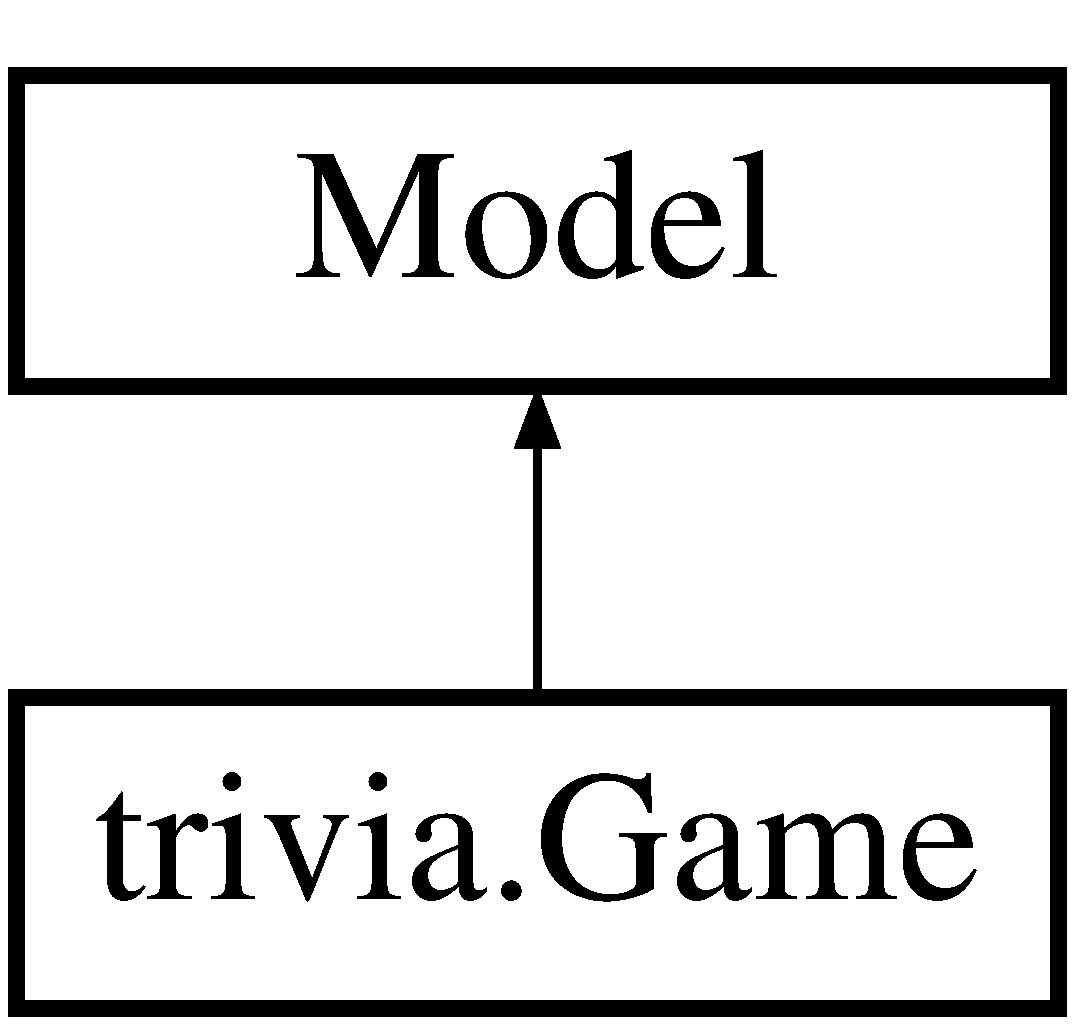
\includegraphics[height=2.000000cm]{classtrivia_1_1Game}
\end{center}
\end{figure}
\subsection*{Public Member Functions}
\begin{DoxyCompactItemize}
\item 
\mbox{\hyperlink{classtrivia_1_1Game_ac0ed7c3b89cdb6936ada292648db5165}{Game}} ()
\item 
boolean \mbox{\hyperlink{classtrivia_1_1Game_a541c6b1a5cac82e7bc3ba39feccf22a7}{is\+Closed}} ()
\item 
Hash\+Map \mbox{\hyperlink{classtrivia_1_1Game_af7ae2d61676f50cea2d5cd07fe37713f}{close\+Game}} ()
\item 
\mbox{\hyperlink{classtrivia_1_1Game_a66e59862c017262e9294558a9e024cbe}{Game}} (\mbox{\hyperlink{classtrivia_1_1User}{User}} unico\+Usuario)
\item 
\mbox{\hyperlink{classtrivia_1_1Game_a03c33ebd51af0b2137101ac28e5b2536}{Game}} (\mbox{\hyperlink{classtrivia_1_1User}{User}} user1, \mbox{\hyperlink{classtrivia_1_1User}{User}} user2)
\item 
Hash\+Map \mbox{\hyperlink{classtrivia_1_1Game_a7b5d8f58e7646f91e21f0182d985960a}{obtener\+Pregunta}} (\mbox{\hyperlink{classtrivia_1_1User}{User}} player)
\item 
void \mbox{\hyperlink{classtrivia_1_1Game_ab5041f892c2f683775d09f2eee17e8d2}{respondio\+Correctamente}} (\mbox{\hyperlink{classtrivia_1_1User}{User}} jugador, int veces\+Correctas)
\item 
void \mbox{\hyperlink{classtrivia_1_1Game_a9cc89954f712f9423034b39cc0b13981}{initialize\+Players}} ()
\item 
\mbox{\Hypertarget{classtrivia_1_1Game_a7ab103e6a0b31ede06021ab65a9cde31}\label{classtrivia_1_1Game_a7ab103e6a0b31ede06021ab65a9cde31}} 
int {\bfseries get\+Cant\+Usuarios} ()
\item 
\mbox{\Hypertarget{classtrivia_1_1Game_a011392205502ca7e6be98ac42b2647d3}\label{classtrivia_1_1Game_a011392205502ca7e6be98ac42b2647d3}} 
\mbox{\hyperlink{classtrivia_1_1User}{User}} {\bfseries get\+Player1} ()
\item 
\mbox{\Hypertarget{classtrivia_1_1Game_a509143fb3810d089e542b241841d1a3e}\label{classtrivia_1_1Game_a509143fb3810d089e542b241841d1a3e}} 
\mbox{\hyperlink{classtrivia_1_1User}{User}} {\bfseries get\+Player2} ()
\item 
\mbox{\Hypertarget{classtrivia_1_1Game_afefdce3a9a90710fd816910d50679e6a}\label{classtrivia_1_1Game_afefdce3a9a90710fd816910d50679e6a}} 
void {\bfseries set\+Player1} (\mbox{\hyperlink{classtrivia_1_1User}{User}} player)
\item 
\mbox{\Hypertarget{classtrivia_1_1Game_afcf7f65afe4042216dea76c9a95c49c4}\label{classtrivia_1_1Game_afcf7f65afe4042216dea76c9a95c49c4}} 
void {\bfseries set\+Player2} (\mbox{\hyperlink{classtrivia_1_1User}{User}} player)
\item 
\mbox{\Hypertarget{classtrivia_1_1Game_a8bae3bf163c788ab952ea4d518203bde}\label{classtrivia_1_1Game_a8bae3bf163c788ab952ea4d518203bde}} 
void {\bfseries set\+Cant\+Usuarios} (int cantidad)
\end{DoxyCompactItemize}
\subsection*{Static Public Member Functions}
\begin{DoxyCompactItemize}
\item 
static void \mbox{\hyperlink{classtrivia_1_1Game_acff76e402d22f7d1b17c2f8c878ec9fc}{init\+Game}} (\mbox{\hyperlink{classtrivia_1_1Game}{Game}} game, \mbox{\hyperlink{classtrivia_1_1User}{User}} user)
\item 
static void \mbox{\hyperlink{classtrivia_1_1Game_ac78e285c8f07840b96bd4bba0d65869b}{init\+Game}} (\mbox{\hyperlink{classtrivia_1_1Game}{Game}} game, int cant\+Preguntas, \mbox{\hyperlink{classtrivia_1_1User}{User}} user1, \mbox{\hyperlink{classtrivia_1_1User}{User}} user2)
\end{DoxyCompactItemize}


\subsection{Detailed Description}
Clase que permite administrar una partida del juego. \begin{DoxyAuthor}{Author}
Maria, Santiago; Rivero, Matias. 
\end{DoxyAuthor}
\begin{DoxyVersion}{Version}
0.\+3 
\end{DoxyVersion}


\subsection{Constructor \& Destructor Documentation}
\mbox{\Hypertarget{classtrivia_1_1Game_ac0ed7c3b89cdb6936ada292648db5165}\label{classtrivia_1_1Game_ac0ed7c3b89cdb6936ada292648db5165}} 
\index{trivia\+::\+Game@{trivia\+::\+Game}!Game@{Game}}
\index{Game@{Game}!trivia\+::\+Game@{trivia\+::\+Game}}
\subsubsection{\texorpdfstring{Game()}{Game()}\hspace{0.1cm}{\footnotesize\ttfamily [1/3]}}
{\footnotesize\ttfamily trivia.\+Game.\+Game (\begin{DoxyParamCaption}{ }\end{DoxyParamCaption})\hspace{0.3cm}{\ttfamily [inline]}}

Constructor basico de la clase.-\/ \begin{DoxyAuthor}{Author}
Maria, Santiago; Rivero, Matias. 
\end{DoxyAuthor}
\mbox{\Hypertarget{classtrivia_1_1Game_a66e59862c017262e9294558a9e024cbe}\label{classtrivia_1_1Game_a66e59862c017262e9294558a9e024cbe}} 
\index{trivia\+::\+Game@{trivia\+::\+Game}!Game@{Game}}
\index{Game@{Game}!trivia\+::\+Game@{trivia\+::\+Game}}
\subsubsection{\texorpdfstring{Game()}{Game()}\hspace{0.1cm}{\footnotesize\ttfamily [2/3]}}
{\footnotesize\ttfamily trivia.\+Game.\+Game (\begin{DoxyParamCaption}\item[{\mbox{\hyperlink{classtrivia_1_1User}{User}}}]{unico\+Usuario }\end{DoxyParamCaption})\hspace{0.3cm}{\ttfamily [inline]}}

Constructor de un juego Single Player. \begin{DoxyAuthor}{Author}
Maria, Santiago; Rivero, Matias. 
\end{DoxyAuthor}

\begin{DoxyParams}{Parameters}
{\em unico\+Usuario} & Usuario que desea abrir una partida single player. \\
\hline
\end{DoxyParams}
\mbox{\Hypertarget{classtrivia_1_1Game_a03c33ebd51af0b2137101ac28e5b2536}\label{classtrivia_1_1Game_a03c33ebd51af0b2137101ac28e5b2536}} 
\index{trivia\+::\+Game@{trivia\+::\+Game}!Game@{Game}}
\index{Game@{Game}!trivia\+::\+Game@{trivia\+::\+Game}}
\subsubsection{\texorpdfstring{Game()}{Game()}\hspace{0.1cm}{\footnotesize\ttfamily [3/3]}}
{\footnotesize\ttfamily trivia.\+Game.\+Game (\begin{DoxyParamCaption}\item[{\mbox{\hyperlink{classtrivia_1_1User}{User}}}]{user1,  }\item[{\mbox{\hyperlink{classtrivia_1_1User}{User}}}]{user2 }\end{DoxyParamCaption})\hspace{0.3cm}{\ttfamily [inline]}}

Constructor de un juego Multi-\/\+Player. \begin{DoxyAuthor}{Author}
Maria, Santiago; Rivero, Matias. 
\end{DoxyAuthor}

\begin{DoxyParams}{Parameters}
{\em user1} & Usuario que creo el juego multi-\/player. \\
\hline
{\em user2} & Usuario que se unio al juego multi-\/player. \\
\hline
\end{DoxyParams}


\subsection{Member Function Documentation}
\mbox{\Hypertarget{classtrivia_1_1Game_af7ae2d61676f50cea2d5cd07fe37713f}\label{classtrivia_1_1Game_af7ae2d61676f50cea2d5cd07fe37713f}} 
\index{trivia\+::\+Game@{trivia\+::\+Game}!close\+Game@{close\+Game}}
\index{close\+Game@{close\+Game}!trivia\+::\+Game@{trivia\+::\+Game}}
\subsubsection{\texorpdfstring{close\+Game()}{closeGame()}}
{\footnotesize\ttfamily Hash\+Map trivia.\+Game.\+close\+Game (\begin{DoxyParamCaption}{ }\end{DoxyParamCaption})\hspace{0.3cm}{\ttfamily [inline]}}

Metodo que cierra el juego actual y devuelve un map con los datos del ganador y perdedor de la partida. \begin{DoxyAuthor}{Author}
Maria, Santiago; Rivero, Matias. 
\end{DoxyAuthor}
\mbox{\Hypertarget{classtrivia_1_1Game_acff76e402d22f7d1b17c2f8c878ec9fc}\label{classtrivia_1_1Game_acff76e402d22f7d1b17c2f8c878ec9fc}} 
\index{trivia\+::\+Game@{trivia\+::\+Game}!init\+Game@{init\+Game}}
\index{init\+Game@{init\+Game}!trivia\+::\+Game@{trivia\+::\+Game}}
\subsubsection{\texorpdfstring{init\+Game()}{initGame()}\hspace{0.1cm}{\footnotesize\ttfamily [1/2]}}
{\footnotesize\ttfamily static void trivia.\+Game.\+init\+Game (\begin{DoxyParamCaption}\item[{\mbox{\hyperlink{classtrivia_1_1Game}{Game}}}]{game,  }\item[{\mbox{\hyperlink{classtrivia_1_1User}{User}}}]{user }\end{DoxyParamCaption})\hspace{0.3cm}{\ttfamily [inline]}, {\ttfamily [static]}}

Metodo estatico que inicializa un juego multi-\/player con el primer jugador. Lo pone en cola hasta que se una el segundo jugador. \begin{DoxyAuthor}{Author}
Maria, Santiago; Rivero, Matias. 
\end{DoxyAuthor}

\begin{DoxyParams}{Parameters}
{\em game} & Juego que se desea inicializar. \\
\hline
{\em user} & Usuario que busca jugar Multi-\/\+Player. \\
\hline
\end{DoxyParams}
\mbox{\Hypertarget{classtrivia_1_1Game_ac78e285c8f07840b96bd4bba0d65869b}\label{classtrivia_1_1Game_ac78e285c8f07840b96bd4bba0d65869b}} 
\index{trivia\+::\+Game@{trivia\+::\+Game}!init\+Game@{init\+Game}}
\index{init\+Game@{init\+Game}!trivia\+::\+Game@{trivia\+::\+Game}}
\subsubsection{\texorpdfstring{init\+Game()}{initGame()}\hspace{0.1cm}{\footnotesize\ttfamily [2/2]}}
{\footnotesize\ttfamily static void trivia.\+Game.\+init\+Game (\begin{DoxyParamCaption}\item[{\mbox{\hyperlink{classtrivia_1_1Game}{Game}}}]{game,  }\item[{int}]{cant\+Preguntas,  }\item[{\mbox{\hyperlink{classtrivia_1_1User}{User}}}]{user1,  }\item[{\mbox{\hyperlink{classtrivia_1_1User}{User}}}]{user2 }\end{DoxyParamCaption})\hspace{0.3cm}{\ttfamily [inline]}, {\ttfamily [static]}}

Metodo estatico que inicializa un juego multi-\/player con ambos jugadores necesarios.-\/ El estado del juego pasa a ser activo. \begin{DoxyAuthor}{Author}
Maria, Santiago; Rivero, Matias. 
\end{DoxyAuthor}

\begin{DoxyParams}{Parameters}
{\em game} & Juego que se inicializa. \\
\hline
{\em user1} & Jugador 1 de la partida. \\
\hline
{\em user2} & Jugador 2 de la partida. \\
\hline
\end{DoxyParams}
\mbox{\Hypertarget{classtrivia_1_1Game_a9cc89954f712f9423034b39cc0b13981}\label{classtrivia_1_1Game_a9cc89954f712f9423034b39cc0b13981}} 
\index{trivia\+::\+Game@{trivia\+::\+Game}!initialize\+Players@{initialize\+Players}}
\index{initialize\+Players@{initialize\+Players}!trivia\+::\+Game@{trivia\+::\+Game}}
\subsubsection{\texorpdfstring{initialize\+Players()}{initializePlayers()}}
{\footnotesize\ttfamily void trivia.\+Game.\+initialize\+Players (\begin{DoxyParamCaption}{ }\end{DoxyParamCaption})\hspace{0.3cm}{\ttfamily [inline]}}

Metodo que inicializa los atributos de los jugadores antes de iniciar el juego. \begin{DoxyAuthor}{Author}
Maria, Santiago; Rivero, Matias. 
\end{DoxyAuthor}
\mbox{\Hypertarget{classtrivia_1_1Game_a541c6b1a5cac82e7bc3ba39feccf22a7}\label{classtrivia_1_1Game_a541c6b1a5cac82e7bc3ba39feccf22a7}} 
\index{trivia\+::\+Game@{trivia\+::\+Game}!is\+Closed@{is\+Closed}}
\index{is\+Closed@{is\+Closed}!trivia\+::\+Game@{trivia\+::\+Game}}
\subsubsection{\texorpdfstring{is\+Closed()}{isClosed()}}
{\footnotesize\ttfamily boolean trivia.\+Game.\+is\+Closed (\begin{DoxyParamCaption}{ }\end{DoxyParamCaption})\hspace{0.3cm}{\ttfamily [inline]}}

Metodo que devuelve True si el juego esta cerrado o inactivo, y False en caso contrario. \begin{DoxyAuthor}{Author}
Maria, Santiago; Rivero, Matias. 
\end{DoxyAuthor}
\mbox{\Hypertarget{classtrivia_1_1Game_a7b5d8f58e7646f91e21f0182d985960a}\label{classtrivia_1_1Game_a7b5d8f58e7646f91e21f0182d985960a}} 
\index{trivia\+::\+Game@{trivia\+::\+Game}!obtener\+Pregunta@{obtener\+Pregunta}}
\index{obtener\+Pregunta@{obtener\+Pregunta}!trivia\+::\+Game@{trivia\+::\+Game}}
\subsubsection{\texorpdfstring{obtener\+Pregunta()}{obtenerPregunta()}}
{\footnotesize\ttfamily Hash\+Map trivia.\+Game.\+obtener\+Pregunta (\begin{DoxyParamCaption}\item[{\mbox{\hyperlink{classtrivia_1_1User}{User}}}]{player }\end{DoxyParamCaption})\hspace{0.3cm}{\ttfamily [inline]}}

Metodo que devuelve una pregunta que puede ser respondida por un usuario con sus respectivas opciones. \begin{DoxyAuthor}{Author}
Maria, Santiago; Rivero, Matias. 
\end{DoxyAuthor}

\begin{DoxyParams}{Parameters}
{\em player} & Jugador que debe responder la pregunta. \\
\hline
\end{DoxyParams}
\mbox{\Hypertarget{classtrivia_1_1Game_ab5041f892c2f683775d09f2eee17e8d2}\label{classtrivia_1_1Game_ab5041f892c2f683775d09f2eee17e8d2}} 
\index{trivia\+::\+Game@{trivia\+::\+Game}!respondio\+Correctamente@{respondio\+Correctamente}}
\index{respondio\+Correctamente@{respondio\+Correctamente}!trivia\+::\+Game@{trivia\+::\+Game}}
\subsubsection{\texorpdfstring{respondio\+Correctamente()}{respondioCorrectamente()}}
{\footnotesize\ttfamily void trivia.\+Game.\+respondio\+Correctamente (\begin{DoxyParamCaption}\item[{\mbox{\hyperlink{classtrivia_1_1User}{User}}}]{jugador,  }\item[{int}]{veces\+Correctas }\end{DoxyParamCaption})\hspace{0.3cm}{\ttfamily [inline]}}

Metodo que actualiza los datos del juego cada vez que un usuario responde correctamente. \begin{DoxyAuthor}{Author}
Maria, Santiago; Rivero, Matias. 
\end{DoxyAuthor}

\begin{DoxyParams}{Parameters}
{\em jugador} & Jugador que respondio correctamente. \\
\hline
{\em veces\+Correctas} & Cantidad de respuestas respondidas correctamente de manera consecutiva. \\
\hline
\end{DoxyParams}


The documentation for this class was generated from the following file\+:\begin{DoxyCompactItemize}
\item 
Game.\+java\end{DoxyCompactItemize}

\hypertarget{classtrivia_1_1Question}{}\section{trivia.\+Question Class Reference}
\label{classtrivia_1_1Question}\index{trivia.\+Question@{trivia.\+Question}}
Inheritance diagram for trivia.\+Question\+:\begin{figure}[H]
\begin{center}
\leavevmode
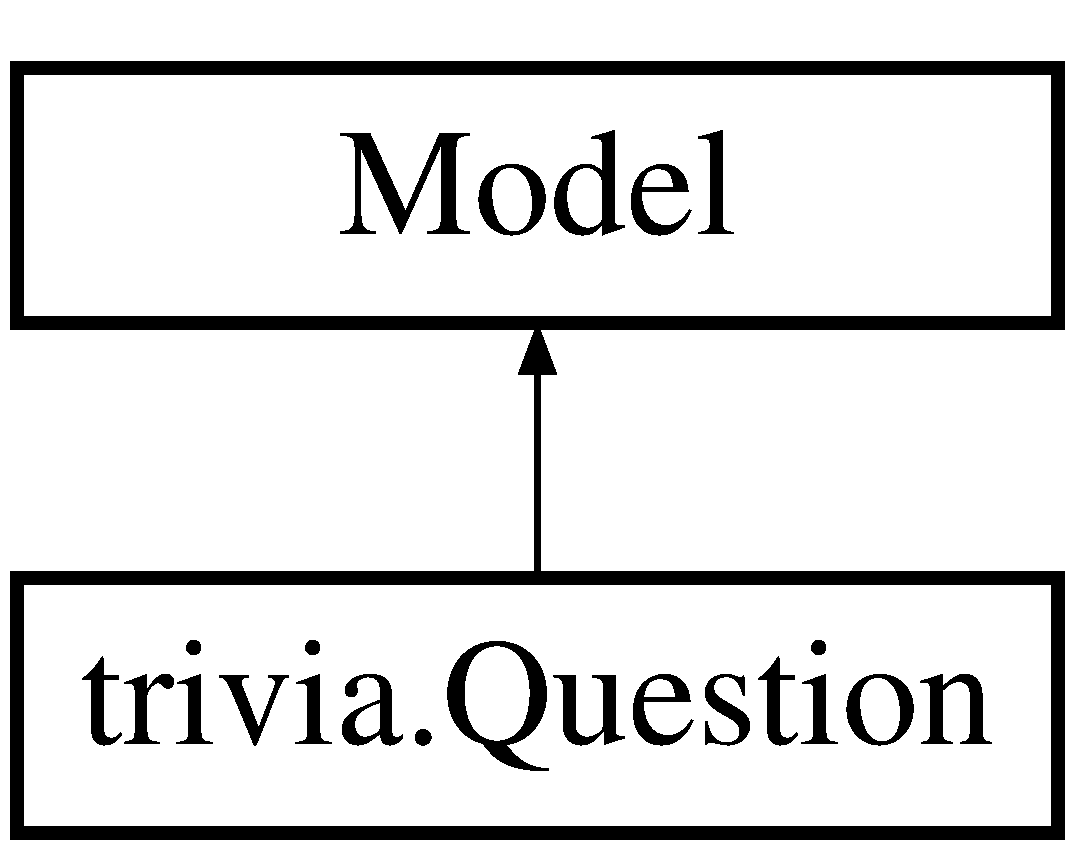
\includegraphics[height=2.000000cm]{classtrivia_1_1Question}
\end{center}
\end{figure}
\subsection*{Public Member Functions}
\begin{DoxyCompactItemize}
\item 
\mbox{\Hypertarget{classtrivia_1_1Question_a13790a82001883a78826412559c5d5a5}\label{classtrivia_1_1Question_a13790a82001883a78826412559c5d5a5}} 
boolean {\bfseries checked} ()
\item 
\mbox{\Hypertarget{classtrivia_1_1Question_a8006494b6b5e147d27b25be464400207}\label{classtrivia_1_1Question_a8006494b6b5e147d27b25be464400207}} 
void {\bfseries check} ()
\item 
\mbox{\Hypertarget{classtrivia_1_1Question_a16043077e35b68a3c68e7101b2f2a85d}\label{classtrivia_1_1Question_a16043077e35b68a3c68e7101b2f2a85d}} 
void {\bfseries un\+Check} ()
\item 
\mbox{\Hypertarget{classtrivia_1_1Question_a52e5fe832dbeb80465259ddb09b52a43}\label{classtrivia_1_1Question_a52e5fe832dbeb80465259ddb09b52a43}} 
void {\bfseries calcular\+Opciones} ()
\item 
\mbox{\Hypertarget{classtrivia_1_1Question_a1dc475316c29c5d9231a8cebcbeb55b6}\label{classtrivia_1_1Question_a1dc475316c29c5d9231a8cebcbeb55b6}} 
int {\bfseries get\+Cant\+Opciones} ()
\end{DoxyCompactItemize}


\subsection{Detailed Description}
Clase \mbox{\hyperlink{classtrivia_1_1Question}{Question}} que representa una pregunta en la base de datos. \begin{DoxyAuthor}{Author}
Maria, Santiago Jose; Rivero, Matias. 
\end{DoxyAuthor}


The documentation for this class was generated from the following file\+:\begin{DoxyCompactItemize}
\item 
Question.\+java\end{DoxyCompactItemize}

\hypertarget{classtrivia_1_1Respondida}{}\section{trivia.\+Respondida Class Reference}
\label{classtrivia_1_1Respondida}\index{trivia.\+Respondida@{trivia.\+Respondida}}
Inheritance diagram for trivia.\+Respondida\+:\begin{figure}[H]
\begin{center}
\leavevmode
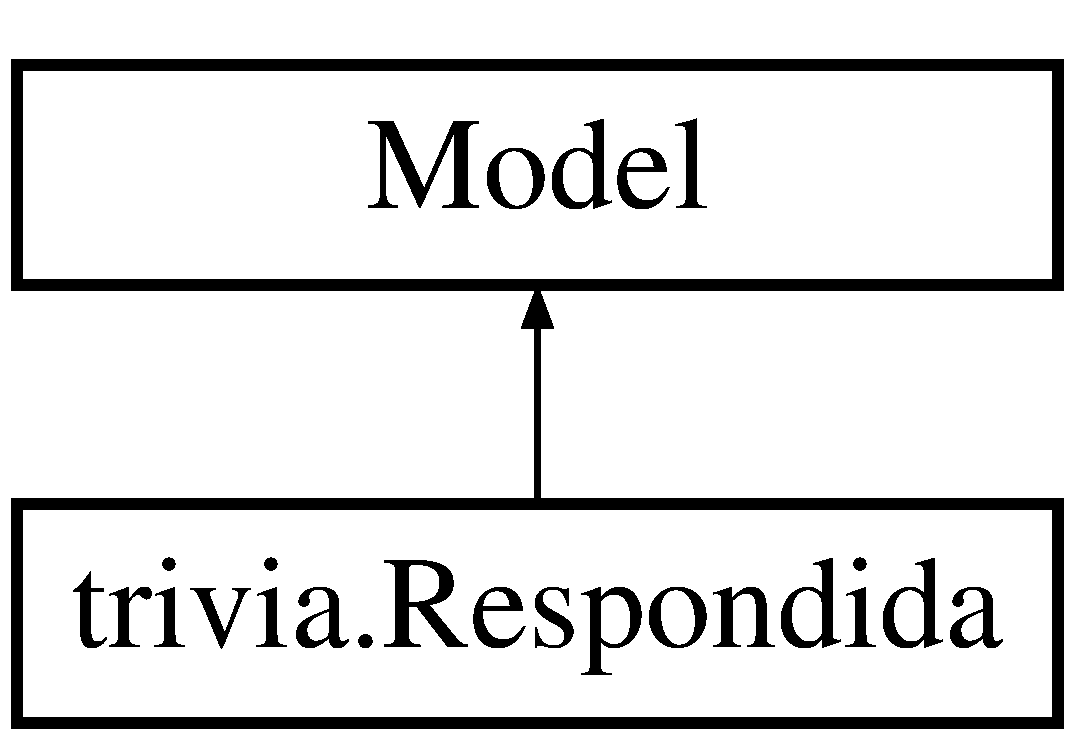
\includegraphics[height=2.000000cm]{classtrivia_1_1Respondida}
\end{center}
\end{figure}


\subsection{Detailed Description}
Clase \mbox{\hyperlink{classtrivia_1_1Respondida}{Respondida}} que representa un elemento de la tabla respondidas, utilizada para mantener registro de las preguntas respondidas por cada usuario. \begin{DoxyAuthor}{Author}
Maria, Santiago Jose; Rivero, Matias. 
\end{DoxyAuthor}


The documentation for this class was generated from the following file\+:\begin{DoxyCompactItemize}
\item 
Respondida.\+java\end{DoxyCompactItemize}

\hypertarget{classtrivia_1_1User}{}\section{trivia.\+User Class Reference}
\label{classtrivia_1_1User}\index{trivia.\+User@{trivia.\+User}}
Inheritance diagram for trivia.\+User\+:\begin{figure}[H]
\begin{center}
\leavevmode
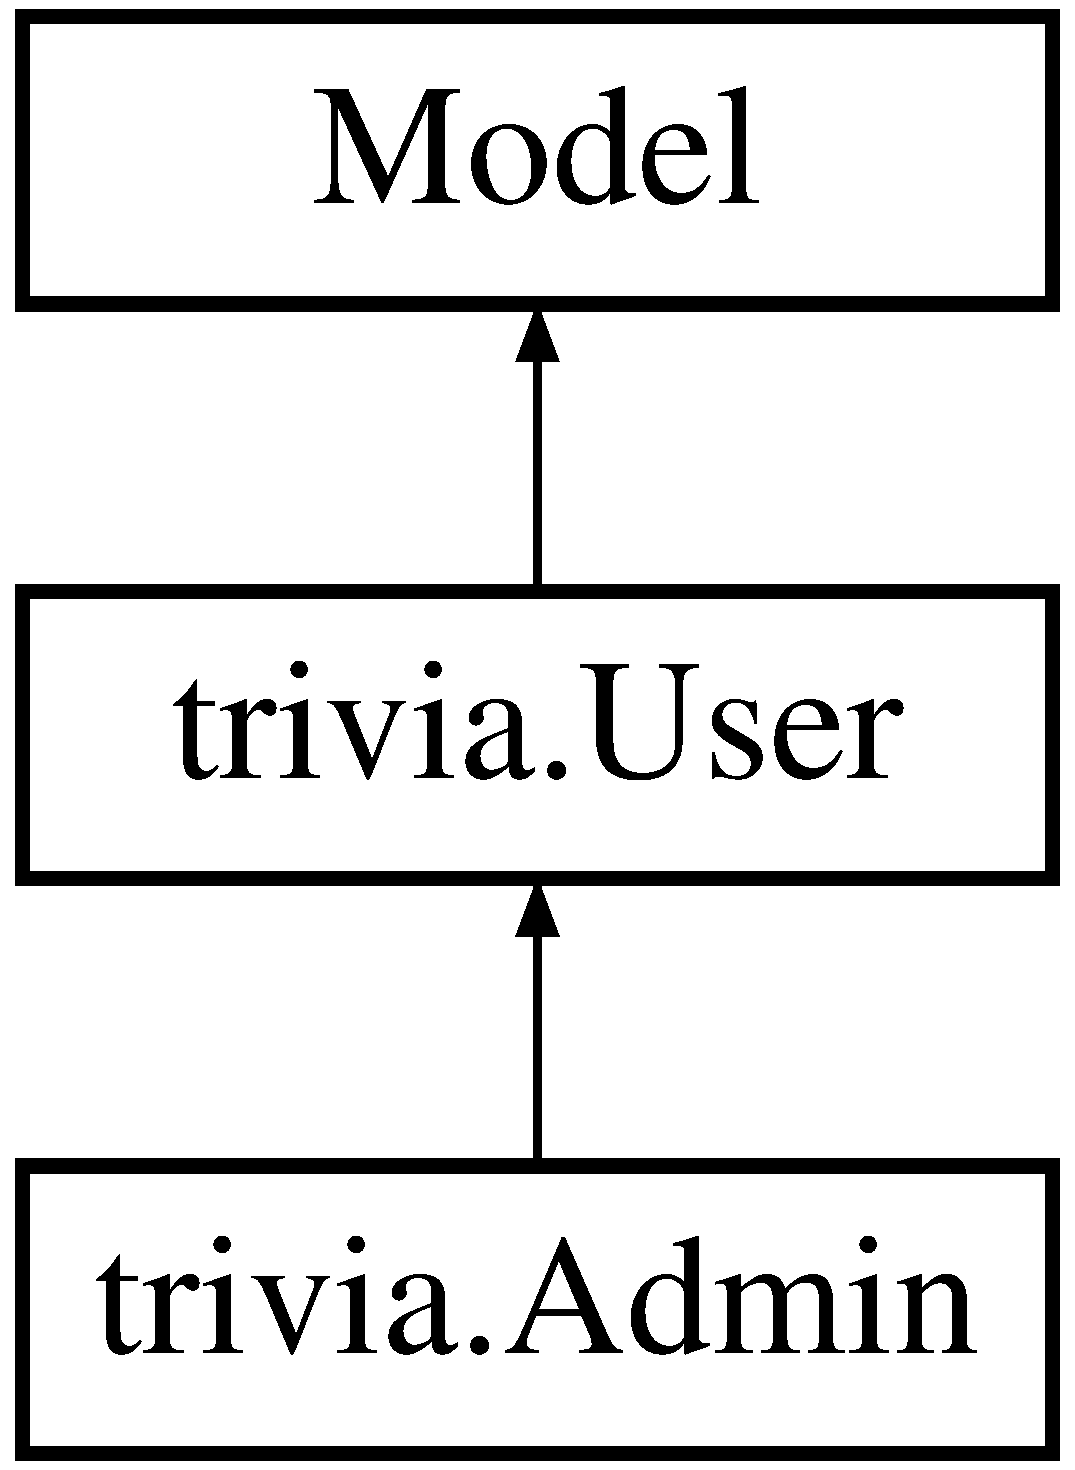
\includegraphics[height=3.000000cm]{classtrivia_1_1User}
\end{center}
\end{figure}
\subsection*{Public Member Functions}
\begin{DoxyCompactItemize}
\item 
\mbox{\Hypertarget{classtrivia_1_1User_a085f90f9229682286b48b07be6aea16b}\label{classtrivia_1_1User_a085f90f9229682286b48b07be6aea16b}} 
{\bfseries User} (String name, String pass)
\item 
\mbox{\Hypertarget{classtrivia_1_1User_a375fc6f8791cb310799536e78f8a3cb3}\label{classtrivia_1_1User_a375fc6f8791cb310799536e78f8a3cb3}} 
void {\bfseries set\+Username} (String new\+Username)
\item 
\mbox{\Hypertarget{classtrivia_1_1User_a89c4c3989287003c38f90aa5b5e4bce0}\label{classtrivia_1_1User_a89c4c3989287003c38f90aa5b5e4bce0}} 
String {\bfseries get\+Username} ()
\item 
\mbox{\Hypertarget{classtrivia_1_1User_a5ced9fd234d3401b005502a4d0645e78}\label{classtrivia_1_1User_a5ced9fd234d3401b005502a4d0645e78}} 
String {\bfseries get\+Password} ()
\item 
\mbox{\Hypertarget{classtrivia_1_1User_a2f7ebdbc1c101511cbaebf58cd0703a3}\label{classtrivia_1_1User_a2f7ebdbc1c101511cbaebf58cd0703a3}} 
int {\bfseries get\+Points} ()
\item 
\mbox{\Hypertarget{classtrivia_1_1User_a751eb03e51be76b13617bcbb461092f4}\label{classtrivia_1_1User_a751eb03e51be76b13617bcbb461092f4}} 
void {\bfseries inc\+Points} ()
\item 
\mbox{\Hypertarget{classtrivia_1_1User_a38c6549660cb21f8e7aacbe54cd188c0}\label{classtrivia_1_1User_a38c6549660cb21f8e7aacbe54cd188c0}} 
void {\bfseries set\+Points} (int puntaje)
\item 
\mbox{\Hypertarget{classtrivia_1_1User_af5ea08746cb8d776250f307bd99340ae}\label{classtrivia_1_1User_af5ea08746cb8d776250f307bd99340ae}} 
void {\bfseries quitar\+Vida} (int cant\+Preguntas)
\item 
\mbox{\Hypertarget{classtrivia_1_1User_a17f8b7e6e9c874f097e8fa3677cbb620}\label{classtrivia_1_1User_a17f8b7e6e9c874f097e8fa3677cbb620}} 
void {\bfseries recover\+Life} ()
\item 
\mbox{\Hypertarget{classtrivia_1_1User_ade19e7e5e337d87be34cc2ebef96699d}\label{classtrivia_1_1User_ade19e7e5e337d87be34cc2ebef96699d}} 
void {\bfseries initialize\+To\+Play} ()
\item 
\mbox{\Hypertarget{classtrivia_1_1User_a2e20d3420cbed90e7e2c17db020fa0d3}\label{classtrivia_1_1User_a2e20d3420cbed90e7e2c17db020fa0d3}} 
double {\bfseries get\+HP} ()
\end{DoxyCompactItemize}


\subsection{Detailed Description}
Clase \mbox{\hyperlink{classtrivia_1_1User}{User}} que representa un usuario en la base de datos. \begin{DoxyAuthor}{Author}
Maria, Santiago Jose; Rivero, Matias. 
\end{DoxyAuthor}


The documentation for this class was generated from the following file\+:\begin{DoxyCompactItemize}
\item 
User.\+java\end{DoxyCompactItemize}

%--- End generated contents ---

% Index
\backmatter
\newpage
\phantomsection
\clearemptydoublepage
\addcontentsline{toc}{chapter}{Index}
\printindex

\end{document}
